\documentclass{article}
\usepackage[T1]{fontenc}
\usepackage[utf8]{inputenc}
\usepackage[margin=2cm]{geometry}
\usepackage{graphicx}
\usepackage{parskip}
\usepackage{booktabs}
\usepackage{amsmath}

\title{Zadanie 6 - Raport}
\author{Jan Stusio}
\date{Czerwiec 2024}

\begin{document}

\maketitle

\section{Wstęp}
Celem zadania jest implementacja algorytmu Q-Learning oraz analizy wpływu parametrów $\alpha$ (współczynnik uczenia), $\gamma$ (współczynnik dyskontowania) i $\epsilon$ (eksploracja w polityce $\epsilon$-zachłannej) oraz parametr T na rozkładzie Bolzmana na zbieżność algorytmu w środowisku FrozenLake-v1 z biblioteki gym. 

\section{Implementacja}
\subsection{Algorytm Q-Learning}
Algorytm Q-Learning jest metodą uczenia ze wzmocnieniem, która polega na iteracyjnym aktualizowaniu funkcji wartości akcji $Q(S, A)$ na podstawie otrzymanej nagrody i wartości funkcji $Q$ w nowym stanie. Wzór aktualizacji funkcji wartości akcji przedstawia się następująco:

\[
Q^{new}(S_t, A_t) \leftarrow (1 - \alpha) \cdot Q(S_t, A_t) + \alpha (R_{t+1} + \gamma \cdot \max_{a} Q(S_{t+1}, a))
\]

Ja w implementacji zmodyfikowałem ten wzór.

\section{Wyniki}

Pomiary na wynikach są dla siatki 4x4, ponieważ nie udało mi się dobrać parametrów, które by dobrze obrazowały zbieżność algorytmu dla siatki 8x8.

\subsection{Wpływ parametru $\alpha$}
Figure 1
\begin{figure}[h!]
    \centering
    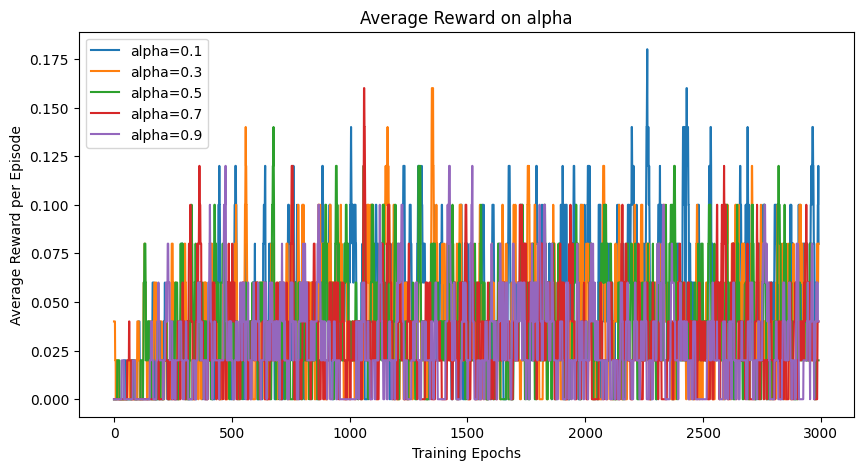
\includegraphics[width=\textwidth]{alpha_impact.png}
    \caption{Wpływ parametru $\alpha$ na zbieżność algorytmu Q-Learning}
    \label{fig:alpha_impact}
\end{figure}
 

\subsection{Wpływ parametru $\gamma$}
Figure 2
\begin{figure}[h!]
    \centering
    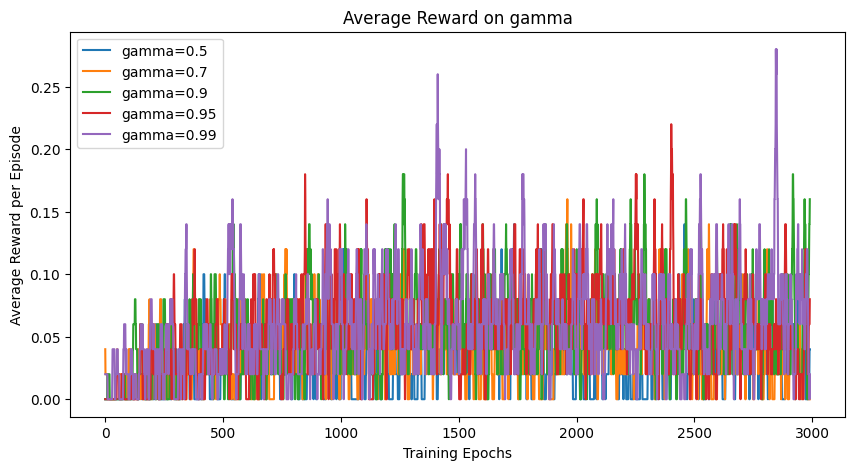
\includegraphics[width=\textwidth]{gamma_impact.png}
    \caption{Wpływ parametru $\gamma$ na zbieżność algorytmu Q-Learning}
    \label{fig:gamma_impact}
\end{figure}
 

\subsection{Wpływ parametru $\epsilon$}
Figure 3
\begin{figure}[h!]
    \centering
    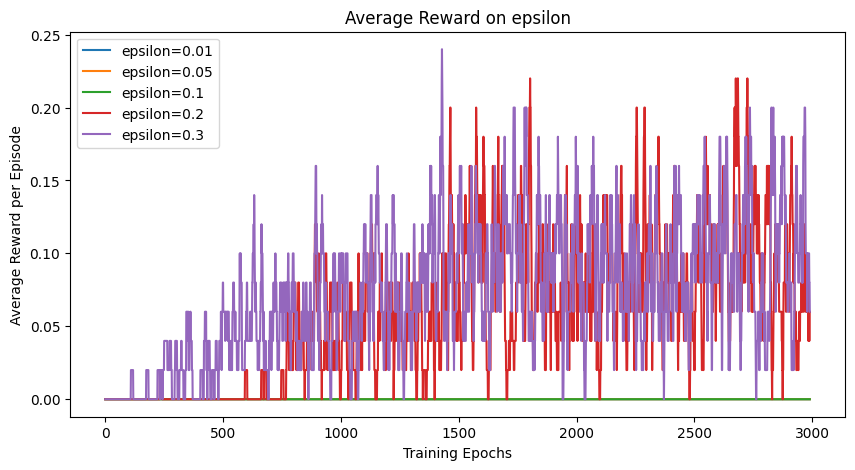
\includegraphics[width=\textwidth]{epsilon_impact.png}
    \caption{Wpływ parametru $\epsilon$ na zbieżność algorytmu Q-Learning}
    \label{fig:epsilon_impact}
\end{figure}
 

\subsection{Wpływ parametru $T$}
Figure 4
\begin{figure}[h!]
    \centering
    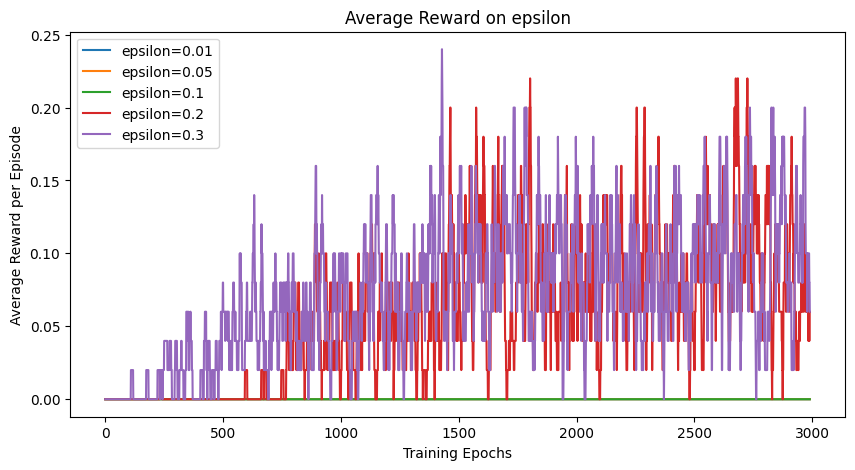
\includegraphics[width=\textwidth]{t_impact.png}
    \caption{Wpływ parametru $T$ na zbieżność algorytmu Q-Learning}
    \label{fig:t_impact}
\end{figure}
 

\subsection{Tabela wyników}
Table 1
\begin{table}[htbp]
    \centering
    \caption{Średnie nagrody w ostatnich 10 epizodach dla różnych wartości badanych parametrów}
    \begin{tabular}{lrrrr}
        \toprule
        Parameter & Value & Mean Reward & Std Reward & Success Count \\
        \midrule
        alpha & 0.100000 & 0.080000 & 0.132665 & 3 \\
        alpha & 0.300000 & 0.080000 & 0.132665 & 3 \\
        alpha & 0.500000 & 0.020000 & 0.060000 & 1 \\
        alpha & 0.700000 & 0.040000 & 0.080000 & 2 \\
        alpha & 0.900000 & 0.040000 & 0.080000 & 2 \\
        gamma & 0.500000 & 0.040000 & 0.080000 & 2 \\
        gamma & 0.700000 & 0.000000 & 0.000000 & 0 \\
        gamma & 0.900000 & 0.160000 & 0.174356 & 6 \\
        gamma & 0.950000 & 0.080000 & 0.097980 & 4 \\
        gamma & 0.990000 & 0.020000 & 0.060000 & 1 \\
        epsilon & 0.010000 & 0.000000 & 0.000000 & 0 \\
        epsilon & 0.050000 & 0.000000 & 0.000000 & 0 \\
        epsilon & 0.100000 & 0.000000 & 0.000000 & 0 \\
        epsilon & 0.200000 & 0.060000 & 0.091652 & 3 \\
        epsilon & 0.300000 & 0.060000 & 0.091652 & 3 \\
        T & 0.500000 & 0.000000 & 0.000000 & 0 \\
        T & 1.000000 & 0.000000 & 0.000000 & 0 \\
        T & 2.000000 & 0.000000 & 0.000000 & 0 \\
        T & 5.000000 & 0.040000 & 0.120000 & 1 \\
        T & 10.000000 & 0.040000 & 0.080000 & 2 \\
        \bottomrule
        \end{tabular}
        
        
\end{table}
 
\pagebreak
   
  .

\pagebreak

  .

\pagebreak

\section{Wnioski}
Na podstawie przeprowadzonych eksperymentów można zauważyć, że wszystkie trzy parametry ($\alpha$, $\gamma$ i $\epsilon$) mają istotny wpływ na zbieżność algorytmu Q-Learning. 

% - Wyższe wartości $\alpha$ prowadzą do szybszego uczenia się, jednak zbyt wysokie wartości mogą powodować niestabilność.
% - Wysokie wartości $\gamma$ sprzyjają długoterminowym nagrodom, co jest korzystne w środowisku z wieloma stanami.
% - Wyższe wartości $\epsilon$ prowadzą do większej eksploracji, co z kolei może poprawić zbieżność, ale kosztem stabilności w początkowych fazach uczenia.

Wyniki potwierdzają, że odpowiedni dobór parametrów jest kluczowy dla efektywnego działania algorytmu Q-Learning.
 
\end{document}
